 %&latex
\documentclass[smaller,a4paper,allowframebreaks]{beamer}
\usepackage{amsmath,amssymb,pdfsync,listings}
\usepackage{verbatim}
\usepackage{graphicx}
\usepackage{truncate}
\usepackage[final]{pdfpages}
\usepackage{times}
\usepackage{pgffor}
\usepackage[english]{babel}

\begin{document}
\title{A (Not So) Simple (Full) Matrix Class}
\frame{\titlepage}

\begin{frame}
\frametitle{Exercise}

\begin{itemize}
%\item Allow the user to specify the problem 
%      and algorithm parameters on the command line
%      rather than in a header
%      \begin{itemize}
%      \item Use GetPot
%      \end{itemize}      
\item Implement a
      library for matrices (and cloumn vectors 
      implemented as 1-column matrices) based on 
      STL containers such as \lstinline[language=C++]{std::vector<>}
      or \lstinline[language=C++]{std::array<>}
      with the following methods/functions
      \begin{itemize}
      \item transpose : $A = A^{T}$
      \item gauss-seidel : solve $A x = b$ iteratively 
      \item (optional) solve : solve $A x = b$ by means of a direct
                    method
      \item operator* : matrix-matrix and matrix-vector
                        multiplication
      \end{itemize}      
\end{itemize}
\end{frame}

\begin{frame}[allowframebreaks]\frametitle{Solution}
\begin{itemize}
\item {\tt matrix-0.1/matrix.\{h,cpp\}}\\[3mm]
\begin{itemize}
\item \lstinline[language=C++]{std::array<>}
      requires the size to be known at compile time,
      in order to make the \lstinline[language=C++]{matrix}
      object configurable at run time we use 
      \lstinline[language=C++]{std::vector<>}\\[3mm]
\item matrices ar organized as \emph{column major}, {\it i.e.}
      $A(i, j) = $ \lstinline[language=C++]{data[i + j * rows ()]}, 
      conversion from 1d to 2d indexing is performed by the utility
      (private) function \lstinline[language=C++]{sub2ind}\\[3mm]
\item access to elements is implemented both in const and non-const
      versions, by overloading \lstinline[language=C++]{operator()} \\[3mm]
\item data is private, \emph{getter methods} expose what is needed to 
      the user, both const and non-const versions are provided \\[3mm]
%\item prototypes of fortran77 functions defined as
%      \lstinline[language=C++]{extern "C" \{...\}}, 
%      assume the compiler adds an underscore (this may change depending 
%      on the compiler), define upper and lower case versions \\[3mm]
%\item use precompiler conditionals to let user select at compile time
%      which implementation to use\\[3mm]
\item naive implementation of matrix-matrix multiplication is slow 
      because it has low \emph{data locality}
      (see below more about memory hierarchy and cache optimized algorithms), 
      simply transposing the left matrix factor improves performance significantly\\[3mm]
%\item BLAS and LAPACK provide cache optimized linear algebra subroutines, optimizations
%      are hardware dependent, the interface of BLAS and LAPACK is fixed, different 
%      implementations with different performance are available\\[3mm]
%      \begin{itemize}
%      \item ATLAS does self tuning via experiments
%      \item OpenBlas has hand-tuned versions for most common architectures
%      \item vendor-specific implementations (Intel MKL, Apple vecLib, \ldots)\\[3mm]
%      \end{itemize} 
\item \lstinline[language=C++]{\#include <ctime>} header provides timing utilities,
      \lstinline[language=C++]{tic ()} and \lstinline[language=C++]{toc (x)} macros
      start and stop the timer (like in Matlab)
\end{itemize}
\item {\tt matrix-0.0/Makefile}\\[3mm]
\begin{itemize}
\item build static and/or shared library\\[3mm]
\item user provided flags are passed on to the preprocessor, compiler and linker
\end{itemize}
%\item {\tt matrix-0.1/test\_*.cpp}\\[3mm]
%\begin{itemize}
%\item for each feature a test to verify consistency and/or performance is provided\\[3mm]
%\item {\tt run\_test.m} builds {\tt test\_matrix\_mult} with various options and
%      compares performance of various implementations\\[3mm]
%\end{itemize}
%\item {\tt fem1d-0.4/fem1d.h}\\[3mm]
%\begin{itemize}
%\item define help text using std::string\\[3mm]
%\item remove config.h\\[3mm]
%\end{itemize}
%\item {\tt fem1d-0.4/fem1d.cpp}\\[3mm]
%\begin{itemize}
%\item define problem/algorithm constants using GetPot methods\\[3mm]
%\item use \lstinline[language=C++]{matrix} objects to define matrices and vectors\\[3mm]
%\end{itemize}
%\item {\tt fem1d-0.4/Makefile}\\[3mm]
%\begin{itemize}
%\item include flags for matrix headers and libraries\\[3mm]
%\end{itemize}
\end{itemize}
\end{frame}

\begin{frame}
\begin{figure}
\begin{center}
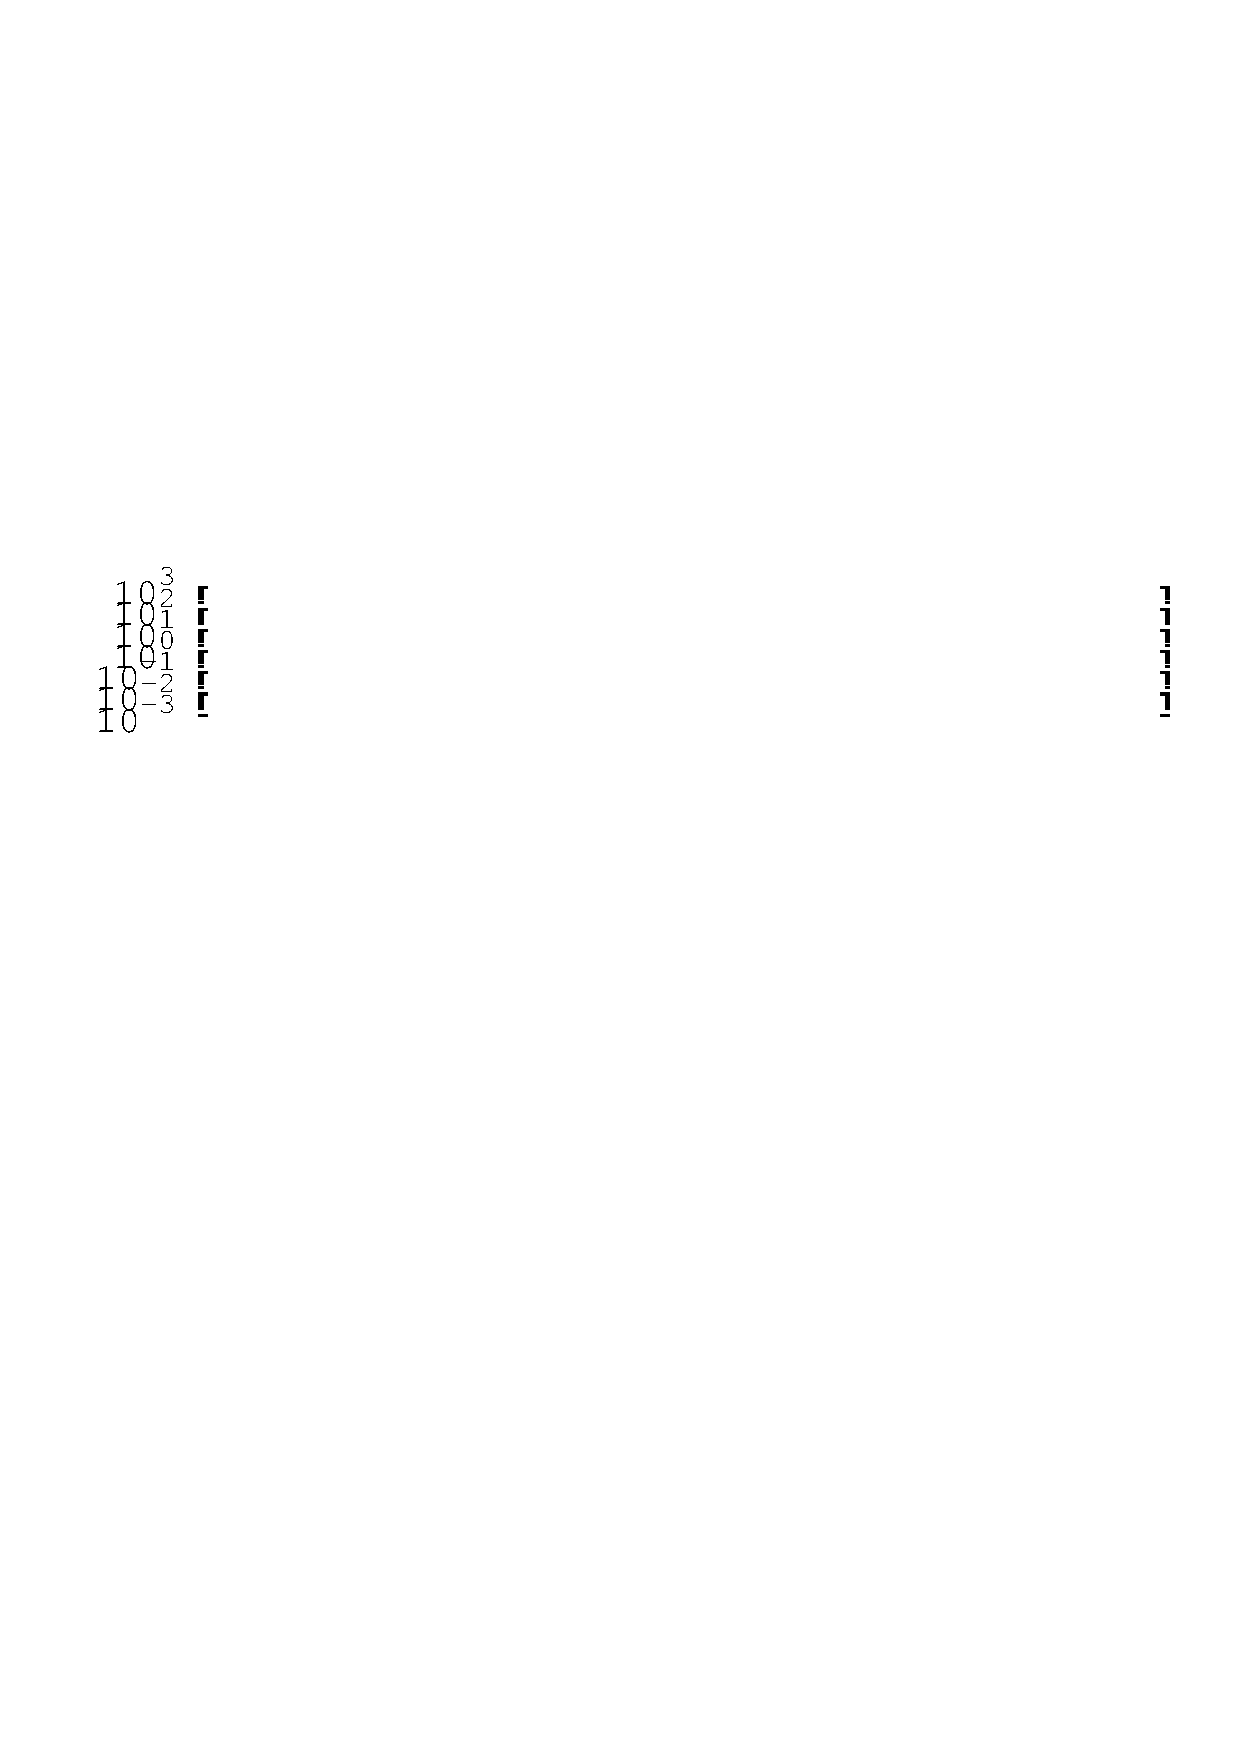
\includegraphics[width=.9\linewidth]{./images/speedup.pdf}
\caption{Performance of the different implementations of the matrix multiplication: 
1) standard (blue), 2) with transpose of first factor (black), 3) DGEMM (red). 
For a matrix of size $2^{11}$ the algorithm 2) is 10 times faster than 1) and algorithm 3) 
is 64 times faster. The comparison was run on MacBook Pro with core2-duo CPU, 
code was compiled with g++ 4.8 and linked to OpenBlas.}
\end{center}
\end{figure}
\end{frame}



\begin{frame}
\frametitle{Matrix Class (Header)}
    \lstset{language=C++,basicstyle=\sffamily\scriptsize}%
    \foreach \n in {1,25,...,85} {%
       \only<+>{%
            \edef\m{\the\numexpr\n+24\relax}%
            \edef\thesubtitle{{Lines \n--\m\ / 85}}%
            \expandafter\framesubtitle\thesubtitle
            \lstinputlisting[numbers=left, numberstyle=\tiny\color{gray},%
                             firstline=\n,lastline=\m,firstnumber=\n]%
                             {../matrix-0.0/matrix.h}%
       }%
    }
\end{frame}

%\begin{frame}
%\frametitle{Matrix Class (Implementation)}
%    \lstset{language=C++,basicstyle=\sffamily\scriptsize}%
%    \foreach \n in {1,25,...,139} {%
%       \only<+>{%
%            \edef\m{\the\numexpr\n+24\relax}%
%            \edef\thesubtitle{{Lines \n--\m\ / 139}}%
%            \expandafter\framesubtitle\thesubtitle
%            \lstinputlisting[numbers=left, numberstyle=\tiny\color{gray},%
%                             firstline=\n,lastline=\m,firstnumber=\n]%
%                             {../matrix-0.0/matrix.cpp}%
%       }%
%    }
%\end{frame}

\begin{frame}
\frametitle{Matrix Class (Test Multiply)}
    \lstset{language=C++,basicstyle=\sffamily\scriptsize}%
            \edef\thesubtitle{{Lines 1--24\ / 24}}%
            \expandafter\framesubtitle\thesubtitle
            \lstinputlisting[numbers=left, numberstyle=\tiny\color{gray},%
                             firstline=1,lastline=24,firstnumber=1]%
                             {../matrix-0.0/test_matrix_mult.cpp}%
\end{frame}

%\begin{frame}
%\frametitle{Matrix Class (Test Gau{\ss}-Seidel)}
%    \lstset{language=C++,basicstyle=\sffamily\scriptsize}%
%    \foreach \n in {1,25,...,37} {%
%       \only<+>{%
%            \edef\m{\the\numexpr\n+24\relax}%
%            \edef\thesubtitle{{Lines \n--\m\ / 37}}%
%            \expandafter\framesubtitle\thesubtitle
%            \lstinputlisting[numbers=left, numberstyle=\tiny\color{gray},%
%                             firstline=\n,lastline=\m,firstnumber=\n]%
%                             {../matrix-0.0/test_gauss_seidel.cpp}%
%       }%
%    }
%\end{frame}

%\begin{frame}
%\frametitle{Matrix Class (Test Solve)}
%    \lstset{language=C++,basicstyle=\sffamily\scriptsize}%
%    \foreach \n in {1,25,...,38} {%
%       \only<+>{%
%            \edef\m{\the\numexpr\n+24\relax}%
%            \edef\thesubtitle{{Lines \n--\m\ / 38}}%
%            \expandafter\framesubtitle\thesubtitle
%            \lstinputlisting[numbers=left, numberstyle=\tiny\color{gray},%
%                             firstline=\n,lastline=\m,firstnumber=\n]%
%                             {../matrix-0.1/test_solve.cpp}%
%       }%
%    }
%\end{frame}

%\begin{frame}
%\frametitle{Matrix Class (run\_test.m)}
%    \lstset{language=Octave,basicstyle=\sffamily\scriptsize}%
%    \foreach \n in {1,25,...,57} {%
%       \only<+>{%
%            \edef\m{\the\numexpr\n+24\relax}%
%            \edef\thesubtitle{{Lines \n--\m\ / 57}}%
%            \expandafter\framesubtitle\thesubtitle
%            \lstinputlisting[numbers=left, numberstyle=\tiny\color{gray},%
%                             firstline=\n,lastline=\m,firstnumber=\n]%
%                             {../matrix-0.1/run_test.m}%
%       }%
%    }
%\end{frame}

\begin{frame}
\frametitle{Matrix Class Library Makefile}
    \lstset{language=make,basicstyle=\sffamily\scriptsize}%
    \foreach \n in {1,25,...,43} {%
       \only<+>{%
            \edef\m{\the\numexpr\n+24\relax}%
            \edef\thesubtitle{{Lines \n--\m\ / 43}}%
            \expandafter\framesubtitle\thesubtitle
            \lstinputlisting[numbers=left, numberstyle=\tiny\color{gray},%
                             firstline=\n,lastline=\m,firstnumber=\n]%
                             {../matrix-0.0/Makefile}%
       }%
    }
\end{frame}

%\begin{frame}
%\frametitle{fem1d main}
%    \lstset{language=C++,basicstyle=\sffamily\scriptsize}%
%    \foreach \n in {1,25,...,79} {%
%       \only<+>{%
%            \edef\m{\the\numexpr\n+24\relax}%
%            \edef\thesubtitle{{Lines \n--\m\ / 79}}%
%            \expandafter\framesubtitle\thesubtitle
%            \lstinputlisting[numbers=left, numberstyle=\tiny\color{gray},%
%                             firstline=\n,lastline=\m,firstnumber=\n]%
%                             {../fem1d-0.4/fem1d.cpp}%
%       }%
%    }
%\end{frame}
%
%\begin{frame}
%\frametitle{fem1d Header}
%    \lstset{language=C++,basicstyle=\sffamily\scriptsize}%
%	\edef\n{1}
%	\edef\m{24}
%    \edef\thesubtitle{{Lines \n--\m\ / 24}}%
%    \expandafter\framesubtitle\thesubtitle
%    \lstinputlisting[numbers=left, numberstyle=\tiny\color{gray},%
%                     firstline=\n,lastline=\m,firstnumber=\n]%
%                             {../fem1d-0.4/fem1d.h}%
%\end{frame}
%
%
%\begin{frame}
%\frametitle{fem1d Executable Makefile}
%    \lstset{language=make,basicstyle=\sffamily\scriptsize}%
%            \edef\thesubtitle{{Lines 1--20\ / 20}}%
%            \expandafter\framesubtitle\thesubtitle
%            \lstinputlisting[numbers=left, numberstyle=\tiny\color{gray},%
%                             firstline=1,lastline=20,firstnumber=1]%
%                             {../fem1d-0.4/Makefile}%
%\end{frame}


\begin{frame}
\frametitle{Memory hierarchy and Cache Optimized Algorithms}
\end{frame}

\begin{frame}
\frametitle{Memory hierarchy and Cache Optimized Algorithms}
insert pages 1-9 of file images/slides.pdf
\end{frame}

\begin{frame}
\frametitle{BLAS and LAPACK}
\end{frame}

\begin{frame}
\frametitle{BLAS and LAPACK}
insert pages 10-20 of file images/slides.pdf
\end{frame}

\end{document}